\section{システム概要}
今回提案するシステムの全体を,図\ref{fig:structure_chart2}に示す.
本システムでは,最初にPCワークを行うアプリケーション利用者(以下,ユーザ)が作業予定の設定を行う.
設定後,ユーザはアプリケーションを起動した状態のまま作業を行う.
その間,起動中のアプリケーションが,ユーザの作業状況を監視し,記録を行う.
記録された情報は,定期的に作業状況として監督者に通知され,監督者はユーザの行動を把握できる.

\begin{figure}[h]
  \begin{center}
  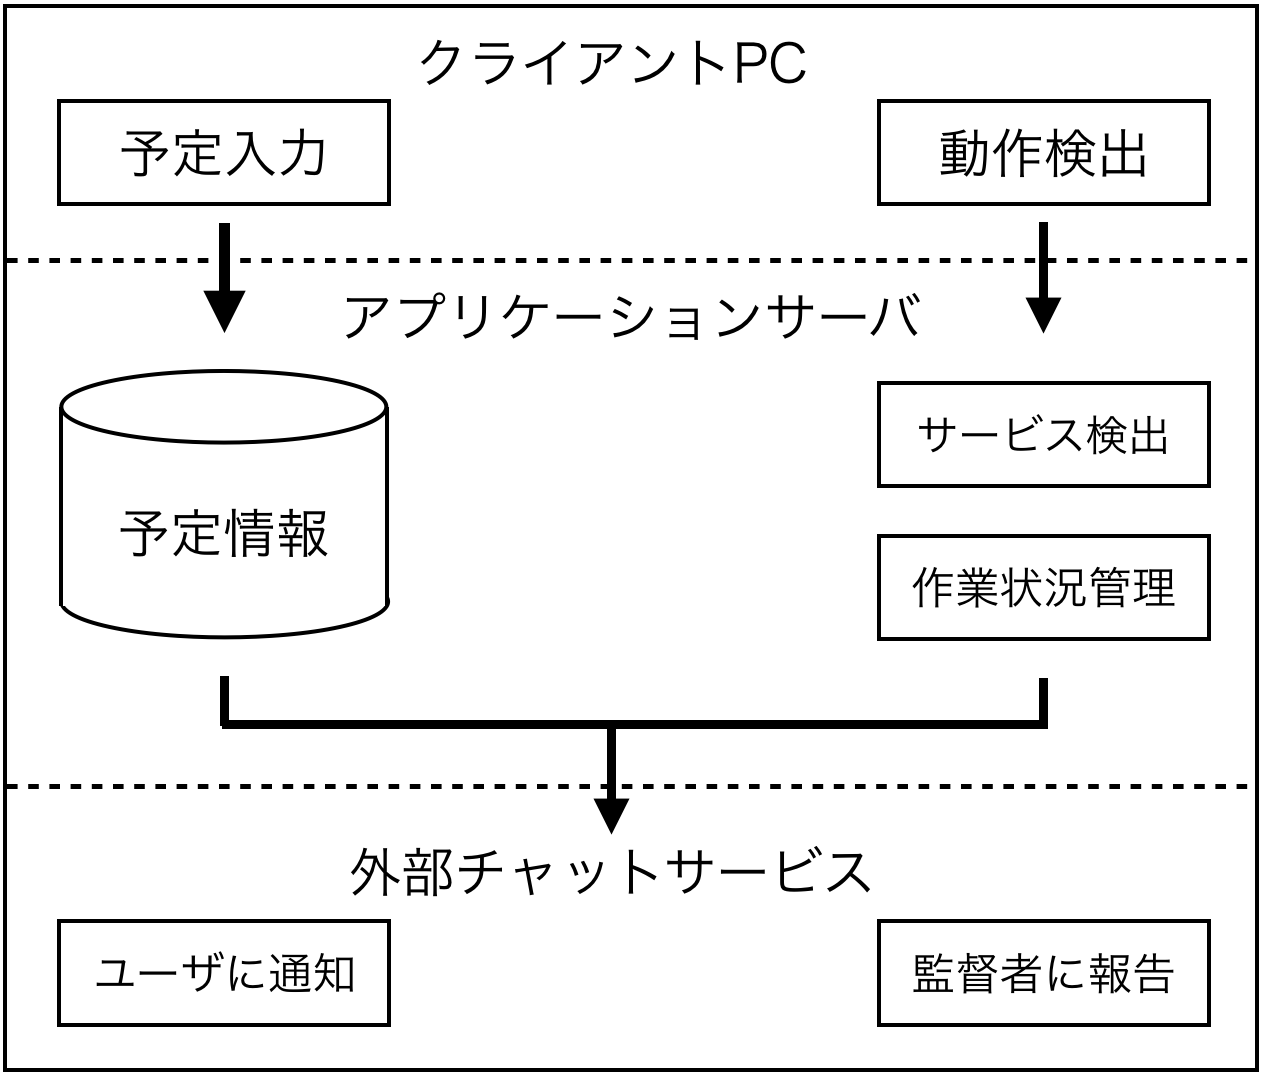
\includegraphics[width=8.0cm]{../graphics/structure_chart2.png}
  \caption{システム構成図}
  \label{fig:structure_chart2}
  \end{center}
\end{figure}

\subsection{アプリケーションによる監視}
アプリケーションの起動状況は,ユーザがアプリケーション起動させておくことで,自動的にサーバに記録される.
また,作業予定になっているもののうち,現在どの作業を行っているのかをユーザが能動的に記録することも可能である.

本研究でのアプリケーションでは,ユーザのPC上で現在表示している画面から,サービスの検出を行う.
まず,アプリケーションが起動している間,ユーザがPC上の画面をキャプチャ画像として自動的に保存する.
その後サーバ上で,それらの画像を解析することにより,ユーザが利用しているサービスの検出を行う.
画像の解析は,Google社のサービスである, Google Cloud Vision API (以下,Vision API)を利用する\cite{visionAPI}.

ユーザの画面キャプチャ画像を Vision API に通すことにより,その画像内に含まれる物体,テキスト情報,サービスのロゴ画像等を検出する.
それらの情報を元に,ユーザが作業に不要なサービスを利用していないかの判別を行う.

\subsection{作業記録の生成}
ユーザは,アプリケーション内で常に自分の作業状況を確認できる.
作業記録は,主に2種類の形式で生成される.

1つは図\ref{fig:activity_table}のように,作業時間をテーブル上に色分けしたものである.
テーブルからは,ユーザが作業を行っていた時間や,作業の予定時間内に作業ができていなかった時間が確認できる.

\begin{figure}[h]
  \begin{center}
  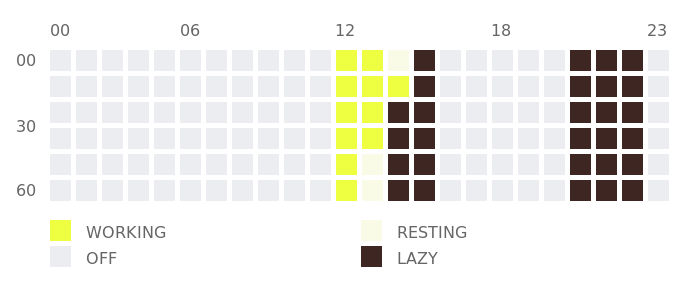
\includegraphics[width=8.0cm]{../graphics/activity_table.png}
  \caption{作業時間のテーブル}
  \label{fig:activity_table}
  \end{center}
\end{figure}

2つ目は,ユーザのアプリケーション内の動作を記録した情報である.
図\ref{fig:activity_log}のように,動作の検出時間と,内容をリスト形式で表示する.
これらの作業記録はすべて監督者への通知でも利用される.

\begin{figure}[h]
  \begin{center}
  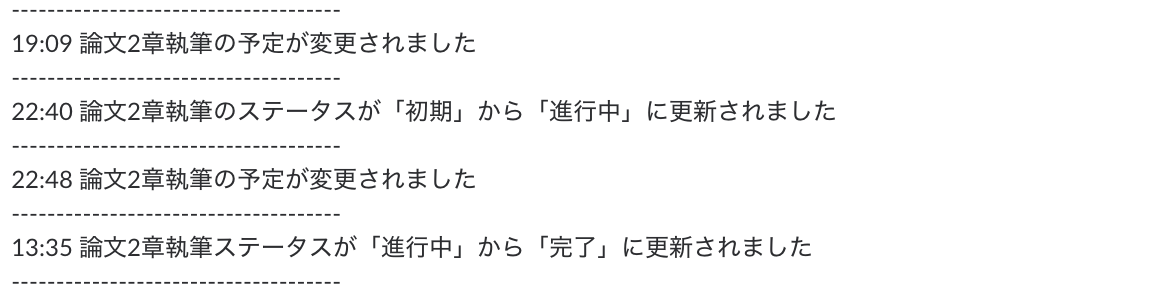
\includegraphics[width=8.0cm]{../graphics/activity_log.png}
  \caption{作業時間のテーブル}
  \label{fig:activity_log}
  \end{center}
\end{figure}
